% 한국어판. 본문 구성은 paper_miccai.tex 와 같다.
% 컴파일: xelatex paper_miccai_ko.tex
\documentclass[runningheads]{llncs}

\usepackage{kotex}
\setmainhangulfont{Malgun Gothic}
\usepackage{graphicx}
\usepackage{booktabs}
\usepackage{amsmath}
\usepackage{url}

\graphicspath{{../results/}}
\renewcommand{\figurename}{그림}
\renewcommand{\tablename}{표}
\renewcommand{\refname}{참고문헌}

\begin{document}

\title{크기별 전문가 분할과 경계 띠 정책 보정을 이용한 뇌종양 MRI 분할}
\titlerunning{뇌종양 MRI의 경계 띠 정책 보정}

\author{안인성\inst{1} \and 한수진\inst{2}}
\authorrunning{안인성, 한수진}
\institute{가천대학교 컴퓨터공학과, 성남, 대한민국
\and
가천대학교 인공지능학과, 성남, 대한민국}

\maketitle

\begin{abstract}
뇌종양 MRI의 Whole Tumor는 단면 크기와 경계 양상이 달라, 하나의 분할 모델로 전 구간을 맞추기 어렵다. 본 연구는 T1ce와 FLAIR를 $128\times128$로 줄인 2차원 슬라이스에서 종양 크기를 분류하고, 크기별 전문가로 초기 마스크를 만든 뒤, 클래스 공통 PPO가 정해진 띠 안의 픽셀을 켜거나 끄는 파이프라인을 제안한다. 면적 300픽셀 미만은 2.5D CaraNet, 300 이상 700 미만은 UNet++, 700 이상은 부종과 종양핵을 나눠 예측한 SegResNet이다. 보정 정책은 하나이며, 전문가 확률 $[0.35,0.65]$인 픽셀 또는 마스크 경계 $\pm2$픽셀을 수정한다. 학습 보상에는 정답을 쓰고, 추론 관측에는 정답이 없다. FLAIR 상대 밝기 제약은 마지막 스텝의 행동에만 둔다.

BraTS 2021 1{,}251명 중 개발 400명(학습 280, 검증 60, 방법 선택 60)을 뺀 851명, 종양 슬라이스 50{,}010장에서 평가했다. 지표는 슬라이스 DSC의 환자 평균이다. 분류기가 전문가를 고르고 임계값을 0.80/0.80/0.50으로 고정한 Stage~2 대비 DSC는 0.8337에서 0.8604로 올랐다(환자 짝 차이 $+0.0267$, 95\% CI $0.0256$--$0.0278$). 검증 60명으로 크기별 임계값을 다시 고른 Stage~2(0.8411)와 비교해도 짝 차이는 $+0.0193$(95\% CI $0.0184$--$0.0202$)이다. 같은 851명에서 검증 60명으로 임계값을 고른 2차원 각색의 DSC는 KAIST 0.8463(임계값 0.40), NVAUTO 0.8576(임계값 0.30)이다. 빈 마스크를 뺀 슬라이스만의 HD95 평균은 NVAUTO 4.184, KAIST 4.224, 제안 방법 4.608픽셀이다. 이 HD95는 방법마다 빠지는 슬라이스가 달라 짝비교로 쓰지 않는다. 본 수치는 BraTS 3차원 리더보드 점수가 아니다. 코드와 실험 기록은 \url{https://github.com/aninsung/2026-summer-Interdepartmental-Academic-Conference}에 있다.

\keywords{뇌종양 분할 \and 자기공명영상 \and 강화학습 \and PPO \and 동적 라우팅 \and 경계 보정}
\end{abstract}

\section{서론}

뇌종양 영역의 분할은 종양 부담을 정량화하고 치료 범위를 정하는 데 쓰인다. MRI에서 종양의 크기, 조영 양상, 부종 경계는 환자마다, 그리고 같은 환자 안에서도 슬라이스마다 달라 단일 백본이 극소 단면과 큰 단면을 동시에 맞추기 어렵다. U-Net 계열은 의료영상 분할의 기본 구조로 자리 잡았으나~\cite{ronneberger2015}, 크기별로 오차 형태가 다르면 초기 마스크의 경계에 체계적인 과소분할이 남을 수 있다. 정밀 방사선 치료에서는 그 경계의 작은 오차도 치료 범위에 영향을 주고, 모든 단면을 사람이 고치는 일은 시간이 많이 든다.

본 연구는 초기 분할과 경계 보정을 나눈다. 분류기가 슬라이스 크기를 고르면 해당 전문가가 확률 맵을 만들고, 하나의 PPO가 애매한 확률 구간과 마스크 경계 주변만 수정한다. 마스크 전체를 다시 그리지 않으므로 전문가가 맞춘 내부는 유지되고, 정책이 손댈 수 있는 곳은 띠 안으로 제한된다. 관측에는 정답이 없고, 정답은 학습 보상에만 쓴다.

기여는 다음 세 가지다.
\begin{enumerate}
\item 소형·중형·대형 전문가로 초기 Whole Tumor 마스크를 만드는 라우팅 분할을 구성하였다.
\item 크기마다 정책을 나누지 않고, 경계 띠 픽셀의 켜기·유지·끄기만 학습하는 PPO 하나를 두었다.
\item 개발에 쓰지 않은 851명에서, 지표의 정의와 주장 범위를 고정한 채 Stage~2 및 2차원 각색과 비교하였다.
\end{enumerate}

\section{관련 연구}

U-Net은 skip connection으로 인코더의 위치 정보와 디코더의 의미 정보를 함께 쓰는 의료영상 분할의 기본 구조다~\cite{ronneberger2015}. 본 연구는 그 계열의 세 모델을 크기 구간에 나눠 배치한다.

\subsection{CaraNet}
CaraNet은 크기가 매우 작은 객체를 정확히 찾도록 설계된 의료영상 분할 모델이다~\cite{lou2023}. 인코더 특징에 문맥 모듈을 두고, Axial Attention과 Reverse Attention을 결합한 모듈로 이미 찾은 영역의 바깥, 곧 놓치기 쉬운 경계 쪽에 주의를 돌린다. 여러 단계의 출력에 감독을 건다. 본 연구에서는 면적 300픽셀 미만의 소형 전문가로 쓴다.

\subsection{SegResNet}
SegResNet은 Encoder--Decoder 구조에 ResNet의 Residual Learning 블록을 결합한 모델이다~\cite{myronenko2018}. 각 블록은 정규화, ReLU, 합성곱을 두 번 거친 뒤 입력을 더한다. 원 논문은 3차원 뇌종양 MRI 분할에 쓰였고, 인코더 출력에서 입력을 복원하는 가지를 정규화로 붙였다. 본 연구에서는 면적 700픽셀 이상의 대형 전문가로 쓰며, 부종과 종양핵을 따로 예측한 뒤 Whole Tumor로 합친다.

\subsection{UNet++}
UNet++는 인코더와 디코더 사이를 중첩된 조밀한 skip connection으로 잇는 U-Net의 고도화 모델이다~\cite{zhou2019}. 같은 해상도의 특징을 여러 단계의 중간 노드로 이어, 인코더와 디코더 특징의 의미 차이를 줄이고 객체 경계선의 분할 정확도를 높인다. 여러 깊이의 출력에 감독을 걸 수 있다. 본 연구에서는 면적 300 이상 700 미만의 중형 전문가로 쓴다.

\subsection{PPO}
PPO(Proximal Policy Optimization)는 정책 경사 계열의 강화학습 알고리즘이다~\cite{schulman2017}. 에이전트가 환경에서 상태를 보고 행동을 고르며 보상을 받는 표본 수집과, 모은 궤적으로 손실을 계산해 정책 신경망을 갱신하는 학습을 번갈아 한다. 새 정책과 이전 정책의 확률 비를 일정 구간으로 자르는(clipping) 목적 함수로 한 번의 갱신 폭을 제한해 학습을 안정시킨다. 같은 궤적을 여러 에폭에 나눠 다시 쓰므로 단순 정책 경사보다 표본을 효율적으로 쓴다. 본 연구에서는 슬라이스 하나를 환경으로, 띠 안 픽셀의 끄기·유지·켜기를 행동으로 둔다.

의료영상에서는 다중 에이전트로 3차원 경계를 반복 수정하는 방법~\cite{liao2020}과 픽셀 단위 강화학습~\cite{furuta2020}이 보고되었다. BraTS 2021에서는 nnU-Net 확장~\cite{luu2021}과 중복 감소를 더한 SegResNet~\cite{myronenko2021}이 상위에 올랐으나, 그 점수는 3차원 패치, 4개 모달리티, 앙상블을 포함한 프로토콜의 점수다. 본 연구의 비교 대상은 같은 2차원·2채널·이진 Whole Tumor 조건으로 각색한 모델이다. 본 연구의 정책은 크기별로 분리하지 않는다. 행동도 외곽선을 한 값만큼 평행 이동하는 방식이 아니라, 정해진 띠 안의 픽셀 레이블을 바꾸는 방식이다. 개발 과정에서는 방위별 거리 이동과 닫힌 윤곽 회귀도 검토했으나, 채택한 구현은 경계 띠 보정이다. 그 검토 수치는 방법 선택 절(\ref{sec:select})과 구분하며, 확정 성능은 \ref{sec:locked}절이다.

\section{방법}
\label{sec:method}

전체 파이프라인은 그림~\ref{fig:pipeline}과 같다. 분류기가 슬라이스 크기를 고르고, 크기별 전문가가 초기 마스크를 만들며, 경계 띠 PPO가 띠 안의 픽셀만 고친다.

\begin{figure}[t]
\centering
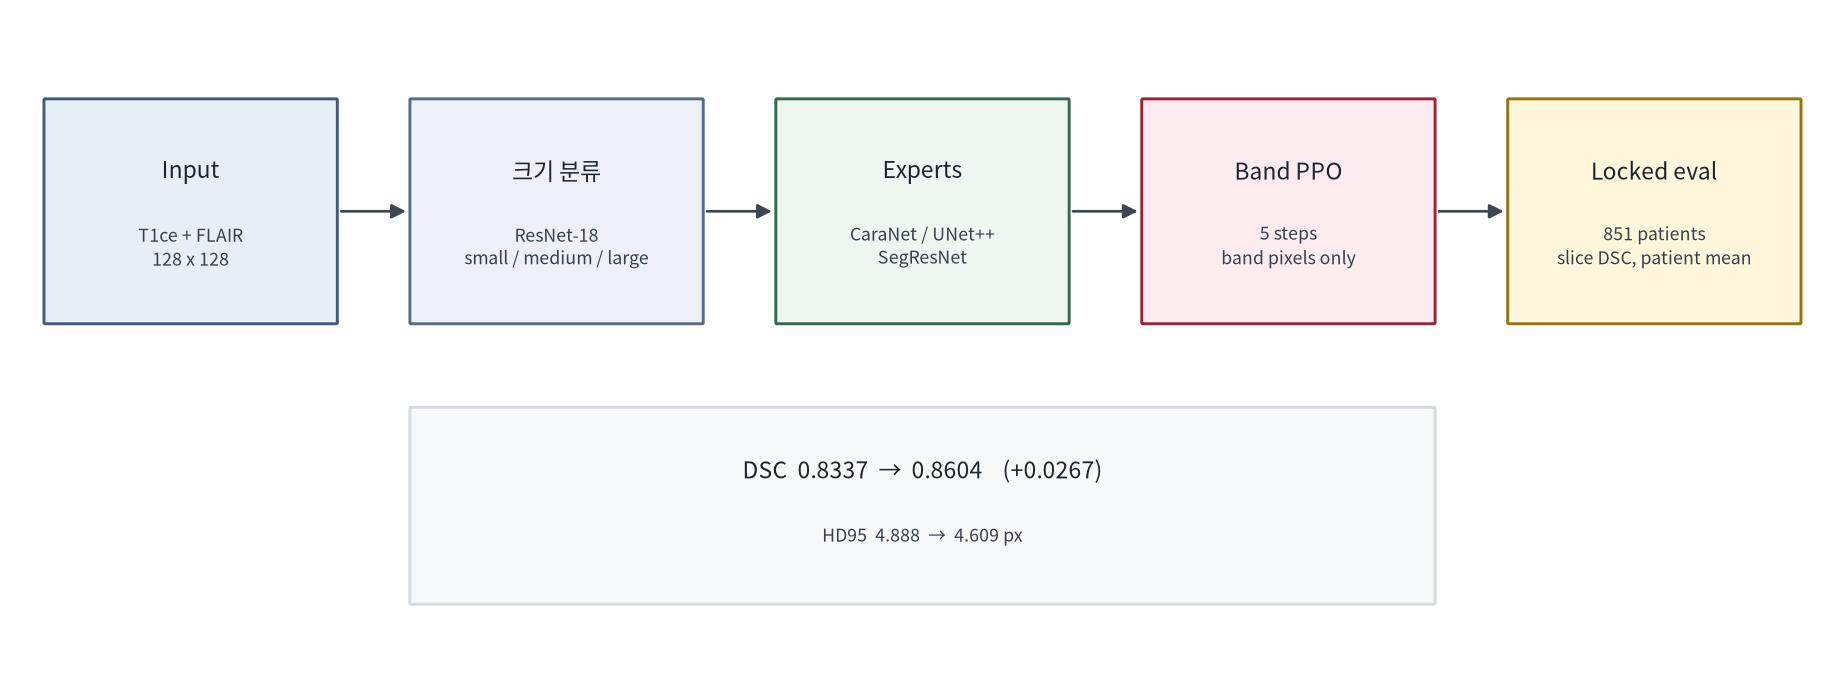
\includegraphics[width=\textwidth]{pipeline_overview.jpg}
\caption{파이프라인. Stage~1은 크기 분류, Stage~2는 크기별 전문가, Stage~3은 경계 띠 PPO, Stage~4는 평가이다.}
\label{fig:pipeline}
\end{figure}

\subsection{데이터와 분할}
입력은 BraTS 2021~\cite{baid2021}의 T1ce와 FLAIR이다. 슬라이스는 $128\times128$로 맞추고, 뇌 영역 안에서 z-score 정규화한 뒤 1--99 퍼센타일로 잘라 $[0,1]$로 맞춘다. 종양 픽셀 비율이 0.2\% 이상인 단면만 학습과 평가에 넣는다. Whole Tumor는 분할 라벨이 0이 아닌 픽셀이다. 크기 기준은 정답 면적이다. 300픽셀 미만은 소형, 300 이상 700 미만은 중형, 700 이상은 대형이다.

환자 단위로 나눈다. 같은 환자의 인접 슬라이스가 학습과 검증에 동시에 들어가지 않는다. 전체 1{,}251명 중 seed 42로 고른 개발 400명은 학습 280, 검증 60, 방법 선택 60이다. 나머지 851명, 종양 슬라이스 50{,}010장은 가중치 학습과 이번 방법 선택에 쓰지 않았다. 다만 Stage~2의 고정 임계값 0.80/0.80/0.50과 연결요소 기준은 이전 프로토콜(같은 seed로 고른 210명 풀)에서 정했고, 그 풀의 148명이 이 851명에 들어 있다. 띠 설계는 이번 방법 선택 60명에서 정했다. 표~\ref{tab:split}이 이 역할을 정리한다.

\begin{table}[t]
\caption{환자 분할.}
\label{tab:split}
\centering
\begin{tabular}{lrl}
\toprule
역할 & 환자 수 & 용도 \\
\midrule
학습 & 280 & 분류기, 전문가, 경계 띠 PPO \\
검증 & 60 & 학습 중 가중치 선택, 베이스라인 임계값 \\
방법 선택 & 60 & 정책 채택. 본문 성능이 아님 \\
확정 평가 & 851 & 한 번 적용한 환자 평균 \\
\bottomrule
\end{tabular}
\end{table}

\subsection{라우팅과 전문가}
분류기는 ImageNet으로 초기화한 ResNet-18이다. 입력은 인접 슬라이스를 붙인 2.5D이고, 첫 합성곱은 RGB 커널을 채널 축으로 합쳐 맞춘다. 면적 경계 $\pm80$픽셀은 학습에서 빼 경계 사례의 라벨 흔들림을 줄인다. 손실은 label smoothing 0.05를 둔 교차엔트로피다. 이번 학습의 검증 정확도는 0.8151이다. 851명 슬라이스에서 분류기 예측이 정답 크기와 맞는 비율은 0.801이다.

추론에서 분류기가 전문가를 고른다. 300픽셀 미만은 2.5D CaraNet이다. 입력이 여섯 채널이고, 아주 작은 정답은 학습에서 더 자주 뽑으며, 1차 예측 뒤 $64\times64$로 확대해 한 번 더 추론한다. 300 이상 700 미만은 중심 슬라이스 두 채널의 UNet++이다. 700 이상은 SegResNet이 부종과 종양핵을 따로 예측한 뒤 Whole Tumor 확률로 합친다. 합치는 식은 $1-(1-p_{\mathrm{ED}})(1-p_{\mathrm{TC}})$이다. 대형 전문가는 전 구간으로 학습하고, 추론에서는 대형으로 분류된 슬라이스에만 쓴다.

확률은 원본과 좌우·상하 반전의 평균이다. 이진화 임계값은 소형·중형·대형이 각각 0.80, 0.80, 0.50이고, 연결요소 최소 크기는 0, 15, 25픽셀이다. 이 임계값은 이번 개발 검증에서 다시 고르지 않고 이전 프로토콜의 값을 고정했다. 검증 60명으로 다시 고른 대조는 \ref{sec:retune}절이다. 전문가 학습은 20에폭, 배치 64, Adam(학습률 $3\times10^{-4}$), 코사인 스케줄, 혼합정밀도다. 손실은 이진 교차엔트로피와 Dice의 합이다. 이번 분할에서 소형 CaraNet의 검증 DSC는 0.8159이다.

학습 때의 전문가 선택은 추론과 다르다. 정책 학습과 저장 에폭 선택은 정답 면적으로 전문가를 골랐다. 851명 평가 슬라이스의 19.9\%는, 그 정답 크기의 학습에 쓰이던 전문가가 아닌 모델의 마스크를 보정한다.

\subsection{경계 띠 PPO}
정책은 하나다. 시작 가중치는 중형 슬라이스만으로 지도학습한 띠 보정 네트워크이다. 네트워크는 폭 32의 소형 U-Net이다. 입력 네 채널은 T1ce, FLAIR, 현재 마스크, 전문가 확률이다. 정답은 관측에 들어가지 않는다. 디코더 끝에서 행동 머리와 가치 머리가 갈라진다. 행동 머리는 픽셀마다 끄기, 유지, 켜기 세 로짓을 내고, 추론은 그 argmax를 쓴다. 가치 머리는 학습에만 쓴다. 띠 밖 로짓은 끄기와 켜기를 막아 유지가 된다.

수정할 수 있는 픽셀은 전문가 확률이 $[0.35,0.65]$인 곳, 또는 현재 마스크 경계에서 2픽셀 안팎이다. 띠 밖은 Stage~2 레이블을 유지한다. 확률이 그 구간에 들어가면 경계에서 멀리 있어도 바뀔 수 있으므로, 수정 범위는 경계 $\pm2$픽셀만이 아니다. 다섯 스텝 동안 확률 맵은 고정하고 마스크만 다음 관측으로 넘긴다.

FLAIR 제약은 마지막 스텝의 행동에만 건다. 그 슬라이스 띠의 평균과 표준편차로 상대 밝기를 내어, 평균보다 어두운 픽셀은 마지막에 켜지 못하고 밝은 픽셀은 마지막에 끄지 못한다. 띠 픽셀이 8개 미만이거나 분산이 없으면 그 슬라이스는 Stage~2를 유지한다. 1--4스텝에는 이 제약이 없으므로, 앞에서 켠 픽셀을 마지막 스텝이 항상 되돌리지는 못한다. 최종 마스크가 FLAIR 규칙을 만족한다고 보지 않는다. DSC가 내려도 초기 마스크로 되돌리지 않는다.

보상은 학습에만 정답을 쓴다. 뒤집은 픽셀이 정답과 같으면 $+1$, 다르면 $-1$이다. 그 스텝에서 양쪽 마스크가 비어 있지 않아 HD95를 계산할 수 있으면, HD95 감소량에 0.25를 곱한 값을 뒤집은 픽셀마다 더한다. HD95 항의 합은 뒤집힌 픽셀 수에 비례한다. 띠 픽셀만으로 GAE를 계산한다. PPO 클립은 0.1, 할인 0.9, GAE $\lambda$는 0.95, 엔트로피 계수 0.001, 가치 계수 0.5이다. 옵티마이저는 AdamW이고 행동 학습률은 $1\times10^{-5}$, 가치 학습률은 $1\times10^{-4}$이다. 에폭은 6, PPO 내부 에폭은 2, 배치는 16이다. 세 크기 클래스를 한 배치에 섞는다.

저장 에폭은 정답 면적 라우팅의 검증에서 macro DSC가 Stage~2 이상이고 macro HD95가 가장 낮은 에폭이다. 저장된 모델은 5에폭이며, 검증 macro DSC 0.8972, HD95 3.558이다. 같은 검증의 Stage~2는 DSC 0.8741, HD95 3.838이다.

내부 경로는 그림~\ref{fig:ppo-route}와 같다. 추론은 네 채널 관측으로 띠를 정하고, FLAIR 제약을 마지막 스텝에만 건 뒤 argmax로 다섯 스텝 마스크를 갱신한다. 학습은 정답을 보상에만 쓴다. 배치 16이 다섯 스텝 경로를 돌고, GAE--PPO가 행동 머리와 가치 머리를 갱신한다.

\begin{figure}[t]
\centering
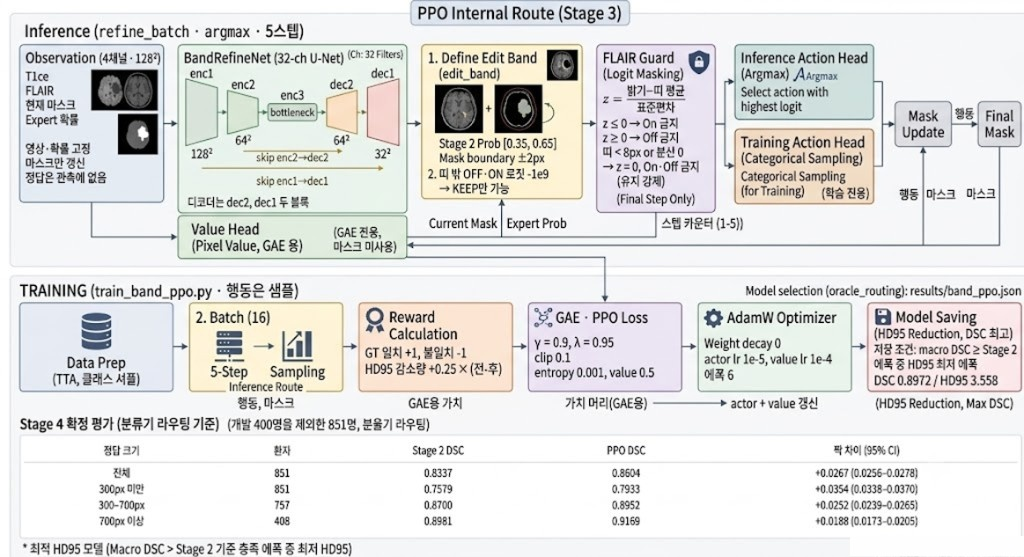
\includegraphics[width=\textwidth]{ppo_internal_route.jpg}
\caption{경계 띠 PPO의 내부 경로. 위는 다섯 스텝 argmax 추론이고, 아래는 보상, GAE--PPO 손실, 행동 머리와 가치 머리의 AdamW 갱신이다. 맨 아래 표는 분류기 라우팅 851명의 확정 평가이다.}
\label{fig:ppo-route}
\end{figure}

\subsection{지표}
주 지표는 슬라이스 DSC의 환자 평균이다. 환자 안에서는 종양 슬라이스를 같은 가중으로 평균하고, 환자 사이도 같은 가중이다. 종양 픽셀 비율 0.2\% 미만인 단면은 평가에 넣지 않는다. 이 값은 BraTS의 3차원 볼륨 Dice가 아니다. Stage~2와의 비교는 환자 짝 차이의 구간으로 한다. 구간은 환자 단위 bootstrap 2{,}000회의 2.5--97.5 백분위이다.

HD95는 같은 $128\times128$ 격자에서 두 윤곽의 95\% 표면 거리이고 단위는 픽셀이다. 밀리미터가 아니다. 예측과 정답 중 한쪽이 비면 그 슬라이스를 HD95 평균에서 빼는데, 방법이 서로 다른 슬라이스를 뺄 수 있다. 환자 수가 같더라도 같은 슬라이스 집합의 짝비교가 아니므로 본문 주장으로 쓰지 않는다. 표에 적힌 HD95는 그 정의로 계산된 기술 평균이다.

크기 행은 환자군이 아니다. 정답 면적이 그 구간에 들어오는 슬라이스만 모아, 그런 슬라이스가 있는 환자의 평균을 낸다. 851명 모두가 300픽셀 미만 슬라이스를 가지므로 그 행의 환자 수는 851이다. 이것은 소형 종양만 있는 환자군이 아니다. 300--700픽셀 행은 757명, 700픽셀 이상 행은 408명이고 같은 환자가 두 행 이상에 들어간다. 행의 환자 수를 더하면 안 된다. 구간별 슬라이스 수는 소형 19{,}077, 중형 19{,}907, 대형 11{,}026이다.

\section{실험}

\subsection{설정}
확정 평가는 개발 400명을 뺀 851명이다. 라우팅은 분류기이고, 전문가는 테스트 시점 증강 뒤 임계값 0.80/0.80/0.50과 연결요소 제거를 거친다. 그 마스크에 경계 띠 PPO를 다섯 스텝 적용한다. 학습과 이 평가는 결정적 연산 모드를 끄고 시드 42로 돌렸다. 수치는 이 학습 실행 한 번이다.

방법 선택에 쓴 60명은 확정 평가에 넣지 않았다. 그 집합의 라우팅은 정답 면적이다. 따라서 \ref{sec:select}절의 DSC를 \ref{sec:locked}절과 나란히 읽어 성능이 올랐거나 내렸다고 해석하지 않는다. 집합, 라우팅, 집계가 다르다.

내부 비교는 같은 분류기, 같은 전문가, 같은 임계값의 Stage~2이다. 경계 띠 PPO만 빠져 있다. 외부 비교는 BraTS 2021 상위 방법의 2차원 각색이다. KAIST 각색은 비대칭 인코더, GroupNorm, 축 방향 attention을 옮긴 nnU-Net 변형이고~\cite{luu2021}, NVAUTO 각색은 SegResNet, InstanceNorm, Barlow Twins 중복 감소를 옮긴 모델이다~\cite{myronenko2021}. 둘 다 단일 모델이 전 크기를 담당하고, 출력은 이진 Whole Tumor 한 채널이다. 입력은 제안 방법과 같이 T1ce와 FLAIR, $128\times128$이다. 3차원 패치, 4개 모달리티, 5겹 앙상블, 대회 후처리는 넣지 않았다. 임계값은 검증 60명의 슬라이스 평균 DSC로만 골랐고, 851명 점수로 고르지 않았다. 탐색 구간은 0.30부터 0.90까지 0.05 간격이며, NVAUTO가 고른 0.30은 그 하한이다. 반전 테스트 시점 증강은 제안 방법에만 있고 두 각색에는 쓰지 않았다.

\subsection{방법 선택}
\label{sec:select}
개발 집합의 방법 선택 60명, 종양 슬라이스 3{,}495장에서 정답 면적으로 전문가를 골랐다. 세 크기 모두 Stage~2보다 DSC가 높고 기록된 HD95 평균이 낮아 이 정책을 채택했다. 표~\ref{tab:select}는 그 채택 기록이다. 논문의 성능 주장은 표~\ref{tab:locked}이다.

\begin{table}[t]
\caption{방법 선택 60명. 정답 면적 라우팅. 확정 성능이 아니다.}
\label{tab:select}
\centering
\begin{tabular}{lcccc}
\toprule
구간 & Stage~2 DSC & PPO DSC & Stage~2 HD95 & PPO HD95 \\
\midrule
소형 & 0.7500 & 0.7846 & 6.640 & 6.393 \\
중형 & 0.9035 & 0.9215 & 3.592 & 2.885 \\
대형 & 0.9223 & 0.9330 & 4.312 & 4.073 \\
전체 & 0.8494 & 0.8721 & 4.905 & 4.474 \\
\bottomrule
\end{tabular}
\end{table}

같은 개발 프로토콜에서 닫힌 윤곽을 반복 이동하는 회귀는 중형·대형 DSC를 Stage~2보다 올렸으나 HD95 평균은 Stage~2보다 낮아지지 않았다. 방위별 거리 이동은 게이트를 풀면 마스크가 무너졌고, 게이트를 두면 Stage~2와 거의 같은 DSC에 머물렀다. 그 실험은 환자 분할이 표~\ref{tab:split}과 다른 기록도 있어 본문 표로 옮기지 않는다. 채택 이유는 표~\ref{tab:select}에서 세 구간 모두 DSC와 기록된 HD95가 Stage~2보다 나았기 때문이다.

\subsection{확정 평가}
\label{sec:locked}
분류기 라우팅으로 851명에 한 번 적용한 결과가 표~\ref{tab:locked}이다. 주 결과는 전체 행이다. 환자 짝 차이 $+0.0267$의 95\% CI는 0을 포함하지 않는다. 아래 세 행은 소형·중형·대형 환자군이 아니다. 본 절의 비교 대상은 고정 임계값의 Stage~2이고, 검증에서 임계값을 다시 고른 대조는 \ref{sec:retune}절이다. 추론은 DSC가 내려간 슬라이스를 되돌리지 않는다.

\begin{table}[t]
\caption{미사용 851명. 분류기 라우팅. 슬라이스 DSC의 환자 평균.}
\label{tab:locked}
\centering
\begin{tabular}{lcccc}
\toprule
정답 면적 & 환자 수 & Stage~2 DSC & PPO DSC & 짝 차이 (95\% CI) \\
\midrule
전체 & 851 & 0.8337 & \textbf{0.8604} & $+0.0267$ (0.0256--0.0278) \\
300px 미만 & 851 & 0.7579 & \textbf{0.7933} & $+0.0354$ (0.0338--0.0370) \\
300--700px & 757 & 0.8700 & \textbf{0.8952} & $+0.0252$ (0.0239--0.0265) \\
700px 이상 & 408 & 0.8981 & \textbf{0.9169} & $+0.0188$ (0.0173--0.0205) \\
\bottomrule
\end{tabular}
\end{table}

차이는 소형 구간에서 가장 크다. 다만 이 행의 851명은 소형 종양 환자가 아니라, 300픽셀 미만 단면이 한 장이라도 있는 환자 전부다. 대형 구간의 차이는 $+0.0188$로 가장 작다. 초기 마스크의 DSC가 이미 0.8981이라 띠 안에서 겹침을 더 올릴 여지가 작다.

같은 파일에 기록된 HD95 평균은 전체 4.888에서 4.609픽셀로 줄었다. 구간별로는 5.801에서 5.697, 4.364에서 3.887, 4.484에서 3.924픽셀이다. 빈 마스크를 빼는 슬라이스가 Stage~2와 PPO에서 달라 이 차이를 짝비교 개선으로 보고하지 않는다.

\subsection{임계값 재선택 대조}
\label{sec:retune}
고정 임계값의 Stage~2는 정밀도 0.883, 재현율 0.820으로 좁은 쪽에 치우친다. 표~\ref{tab:locked}의 차이가 임계값 조정만으로 얻어지는지 보기 위해, 검증 60명에서 분류기 라우팅 기준 크기별 임계값 세 개를 환자 평균 DSC로 함께 다시 골랐다. 탐색 구간은 0.10--0.90, 0.05 간격이고 연결요소 기준은 그대로 둔다. 고른 값은 소형 0.45, 중형 0.80, 대형 0.20이며 구간 끝이 아니다. 검증 DSC는 0.8588에서 0.8650이 되었다. 그 임계값을 851명에 한 번 적용했다. PPO 가중치는 바꾸지 않았고, 고정 임계값 마스크로 학습한 가중치다.

\begin{table}[t]
\caption{미사용 851명. 임계값을 다시 고른 Stage~2와의 짝비교. 수치는 \texttt{results/stage2\_retuned.json}이다.}
\label{tab:retune}
\centering
\small
\begin{tabular}{lcccc}
\toprule
면적 & 고정 Stage~2 & 재선택 & PPO & PPO $-$ 재선택 (95\% CI) \\
\midrule
전체 & 0.8337 & 0.8411 & \textbf{0.8604} & $+0.0193$ (0.0184--0.0202) \\
300px 미만 & 0.7579 & 0.7682 & \textbf{0.7933} & $+0.0251$ (0.0237--0.0265) \\
300--700px & 0.8700 & 0.8790 & \textbf{0.8952} & $+0.0162$ (0.0154--0.0170) \\
700px 이상 & 0.8981 & 0.9014 & \textbf{0.9169} & $+0.0156$ (0.0143--0.0169) \\
\bottomrule
\end{tabular}
\end{table}

임계값 재선택만의 짝 차이는 $+0.0074$($0.0066$--$0.0082$)로, 표~\ref{tab:locked}의 $+0.0267$ 중 약 28\%이다. 나머지 $+0.0193$은 재선택 Stage~2보다도 높고, 세 구간 모두 구간이 0을 포함하지 않는다. 재선택은 재현율을 0.820에서 0.849로 올리는 대신 정밀도를 0.883에서 0.863으로 낮춘다. PPO는 정밀도 0.892, 재현율 0.860으로 둘 다 재선택 Stage~2보다 높다. 재선택 마스크에서 PPO를 시작해도 전체 DSC는 0.8604로 같았다. 띠가 두 임계값 사이의 차이를 대부분 덮기 때문으로 보이며, 그 비율은 따로 재지 않았다.

\subsection{2차원 각색 베이스라인}
같은 851명, 같은 환자 평균으로 KAIST 각색과 NVAUTO 각색을 평가했다. 검증 60명에서 고른 임계값은 KAIST 0.40, NVAUTO 0.30이다. 표~\ref{tab:baselines}는 전체 환자 평균이다. DSC의 주변 구간은 제안 방법 0.8535--0.8672, NVAUTO 0.8510--0.8642, KAIST 0.8398--0.8529이다. 방법 사이 짝 차이는 계산하지 않았다. 제안 방법과 NVAUTO의 주변 구간은 겹친다.

\begin{table}[t]
\caption{851명 환자 평균. 제안 방법과 2차원 각색.}
\label{tab:baselines}
\centering
\begin{tabular}{llcccc}
\toprule
방법 & 임계값 & DSC & HD95 (px) & Precision & Recall \\
\midrule
제안 방법 & 0.80 / 0.80 / 0.50 & 0.8604 & 4.608 & 0.8918 & 0.8600 \\
NVAUTO 각색 & 0.30 & 0.8576 & 4.184 & 0.8836 & 0.8633 \\
KAIST 각색 & 0.40 & 0.8463 & 4.224 & 0.8635 & 0.8642 \\
\bottomrule
\end{tabular}
\end{table}

DSC 평균의 점추정은 제안 방법이 가장 높으나 NVAUTO와 구간이 겹쳐, 두 방법은 비슷한 수준으로 읽는다. 제안 방법만 반전 증강을 쓴 점도 이 차이에 섞여 있다. 제안 방법의 정밀도와 재현율은 0.8918과 0.8600이다. NVAUTO는 정밀도 0.8836, 재현율 0.8633으로 재현율이 조금 더 높다. KAIST는 DSC와 정밀도가 가장 낮다. 빈 마스크를 뺀 HD95 평균은 NVAUTO 4.184, KAIST 4.224, 제안 방법 4.608픽셀로, 이 정의에서는 두 각색이 더 낮다.

표~\ref{tab:bysize}은 정답 면적 구간별 DSC이다. 환자 수의 뜻은 \ref{sec:method}절과 같다. 300픽셀 미만에서는 제안 방법 0.7933, NVAUTO 0.7821, KAIST 0.7664이다. 300--700픽셀과 700픽셀 이상에서는 NVAUTO가 0.8980, 0.9198로 제안 방법 0.8952, 0.9170보다 높다. 제안 방법의 이득은 작은 단면에 몰려 있고, 중형·대형 평균 DSC는 단일 SegResNet 각색이 더 높다. 표~\ref{tab:locked}의 대형 PPO DSC 0.9169와 표~\ref{tab:bysize}의 0.9170은 같은 가중치를 따로 집계한 값이며 소수점 넷째 자리에서 갈린다.

\begin{table}[t]
\caption{정답 면적 구간별 DSC. 괄호는 해당 슬라이스가 있는 환자 수.}
\label{tab:bysize}
\centering
\begin{tabular}{lccc}
\toprule
방법 & 300px 미만 (851) & 300--700px (757) & 700px 이상 (408) \\
\midrule
제안 방법 & 0.7933 & 0.8952 & 0.9170 \\
NVAUTO 각색 & 0.7821 & 0.8980 & 0.9198 \\
KAIST 각색 & 0.7664 & 0.8886 & 0.9160 \\
\bottomrule
\end{tabular}
\end{table}

개발 400명을 뺀 환자에서 고른 같은 슬라이스를 그림~\ref{fig:compare}에 나타냈다. 행은 제안 방법, KAIST 각색, NVAUTO 각색이고 열은 소형, 중형, 대형이다. 각 칸은 그 구간 평균 DSC에 가까운 단면이다. 초록 점선은 정답이다. 정량 주장은 표~\ref{tab:locked}--\ref{tab:bysize}이고, 그림은 경계가 어디서 달라지는지 보기 위한 것이다.

\begin{figure}[t]
\centering
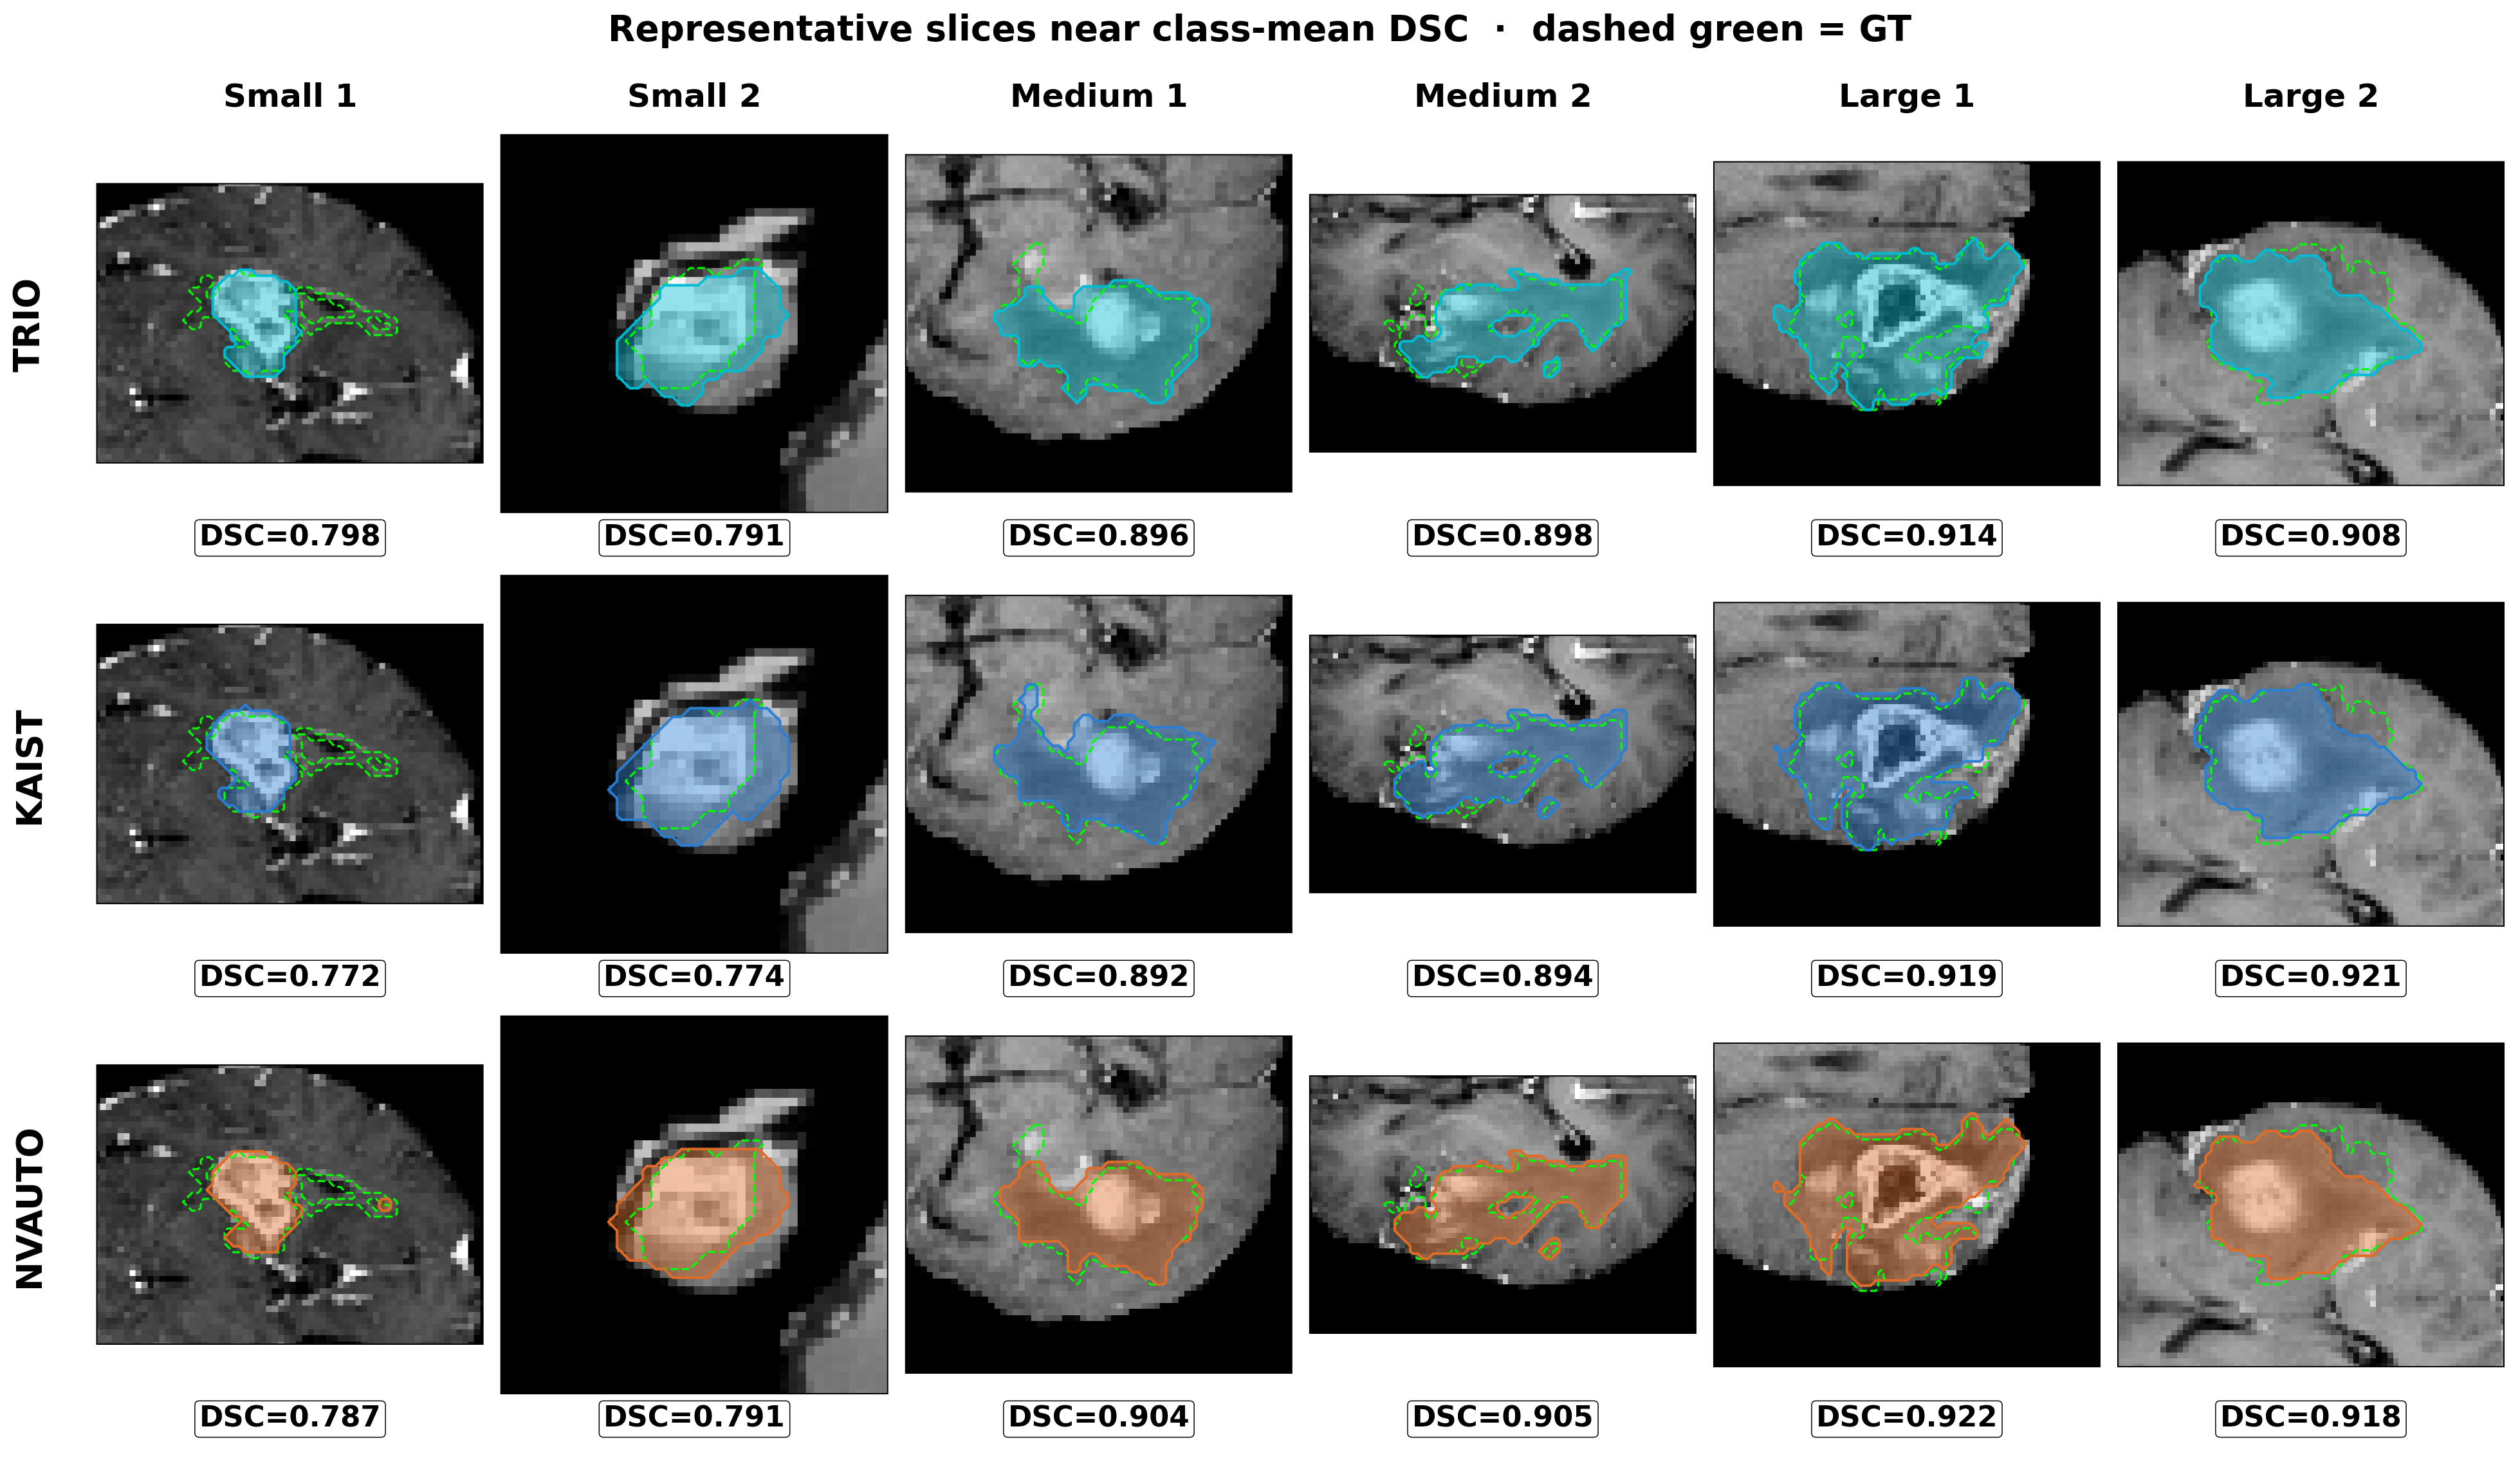
\includegraphics[width=\textwidth]{method_comparison_current_3x6.png}
\caption{미사용 환자의 같은 슬라이스. 위부터 제안 방법, KAIST 각색, NVAUTO 각색. 초록 점선은 정답.}
\label{fig:compare}
\end{figure}

\subsection{단일 백본과 단일 섹터 PPO}
크기별 전문가와 경계 띠를 빼면 성능이 어디까지 떨어지는지 보기 위해, 백본 하나와 섹터 PPO 하나인 세트를 다섯 번 학습했다. 백본은 U-Net, UNet++, UNet+++, Attention U-Net, SegResNet이다. 학습 환자는 표~\ref{tab:split}의 280명이고, 종양 슬라이스 16{,}500장을 크기 구분 없이 모두 쓴다. 에폭은 20, 배치는 32이다. 출력은 이진 Whole Tumor 한 채널이다. 이 SegResNet은 대형 전문가처럼 부종과 종양핵을 나눠 합치지 않는다. 초기 마스크 임계값은 0.5이다. U-Net의 검증 DSC는 0.8834이다.

보정은 경계 띠 PPO가 아니다. 각 백본마다 \texttt{MaskRefinementEnv}의 medium 모드로 PPO를 따로 학습한다. 관측은 영상, 마스크, 확률 세 채널이고, 행동은 $128\times128$을 $5\times8$ 섹터로 나눈 이산 행동이다. 에피소드는 최대 15스텝, 총 스텝은 100{,}000이며 환경 8개가 그 스텝을 나눠 모은다. 정책은 CnnPolicy, 학습률 $3\times10^{-4}$, 엔트로피 계수 0.01이다. 가중치는 \texttt{checkpoints/single\_backbone/}에 있고, TRIO 전문가와 \texttt{band\_ppo.pt}는 덮어쓰지 않았다.

표~\ref{tab:single}과 그림~\ref{fig:single}의 집계는 개발 400명을 뺀 환자 중 seed 7로 고른 48명, 종양 슬라이스 2{,}754장의 슬라이스 평균이다. 환자 평균이 아니고, 표~\ref{tab:locked}--\ref{tab:bysize}의 851명 숫자와 나란히 읽지 않는다. HD95는 양쪽 마스크가 비어 있지 않은 슬라이스만의 슬라이스 평균이다. 그림의 TRIO 열은 같은 48명에 현재 경계 띠 파이프라인을 적용한 값이다. 각 칸은 그 크기 구간의 슬라이스 평균 DSC에 가까운 단면이고, 칸 아래 평균이 표~\ref{tab:single}이다.

\begin{table}[t]
\caption{미사용 48명 표본의 슬라이스 평균. 851명 환자 평균이 아니다.}
\label{tab:single}
\centering
\footnotesize
\setlength{\tabcolsep}{4pt}
\begin{tabular}{lcccccc}
\toprule
방법 & 소형 DSC & 중형 DSC & 대형 DSC & 소형 HD95 & 중형 HD95 & 대형 HD95 \\
\midrule
TRIO (경계 띠) & 0.812 & 0.904 & 0.916 & 4.877 & 3.432 & 3.761 \\
U-Net + PPO & 0.537 & 0.813 & 0.866 & 12.126 & 6.518 & 6.527 \\
UNet++ + PPO & 0.778 & 0.894 & 0.926 & 5.786 & 3.617 & 3.773 \\
UNet+++ + PPO & 0.543 & 0.828 & 0.900 & 10.308 & 5.087 & 4.345 \\
Attention U-Net + PPO & 0.761 & 0.884 & 0.904 & 6.660 & 3.821 & 4.606 \\
SegResNet + PPO & 0.676 & 0.871 & 0.912 & 8.821 & 4.240 & 4.319 \\
\bottomrule
\end{tabular}
\end{table}

이 표본에서 소형 DSC는 TRIO 0.812, UNet++ 0.778, Attention U-Net 0.761 순이다. U-Net과 UNet+++의 소형 DSC는 0.537, 0.543이고 HD95는 12.126, 10.308픽셀이다. 중형과 대형에서는 UNet++가 DSC 0.894, 0.926으로 TRIO 0.904, 0.916과 같은 자리다. 재현은 \texttt{python scripts/eval/plot\_single\_backbone\_grid.py}이고, 파일은 \texttt{results/single\_backbone\_ppo\_grid\_metrics.json}이다.

\begin{figure}[t]
\centering
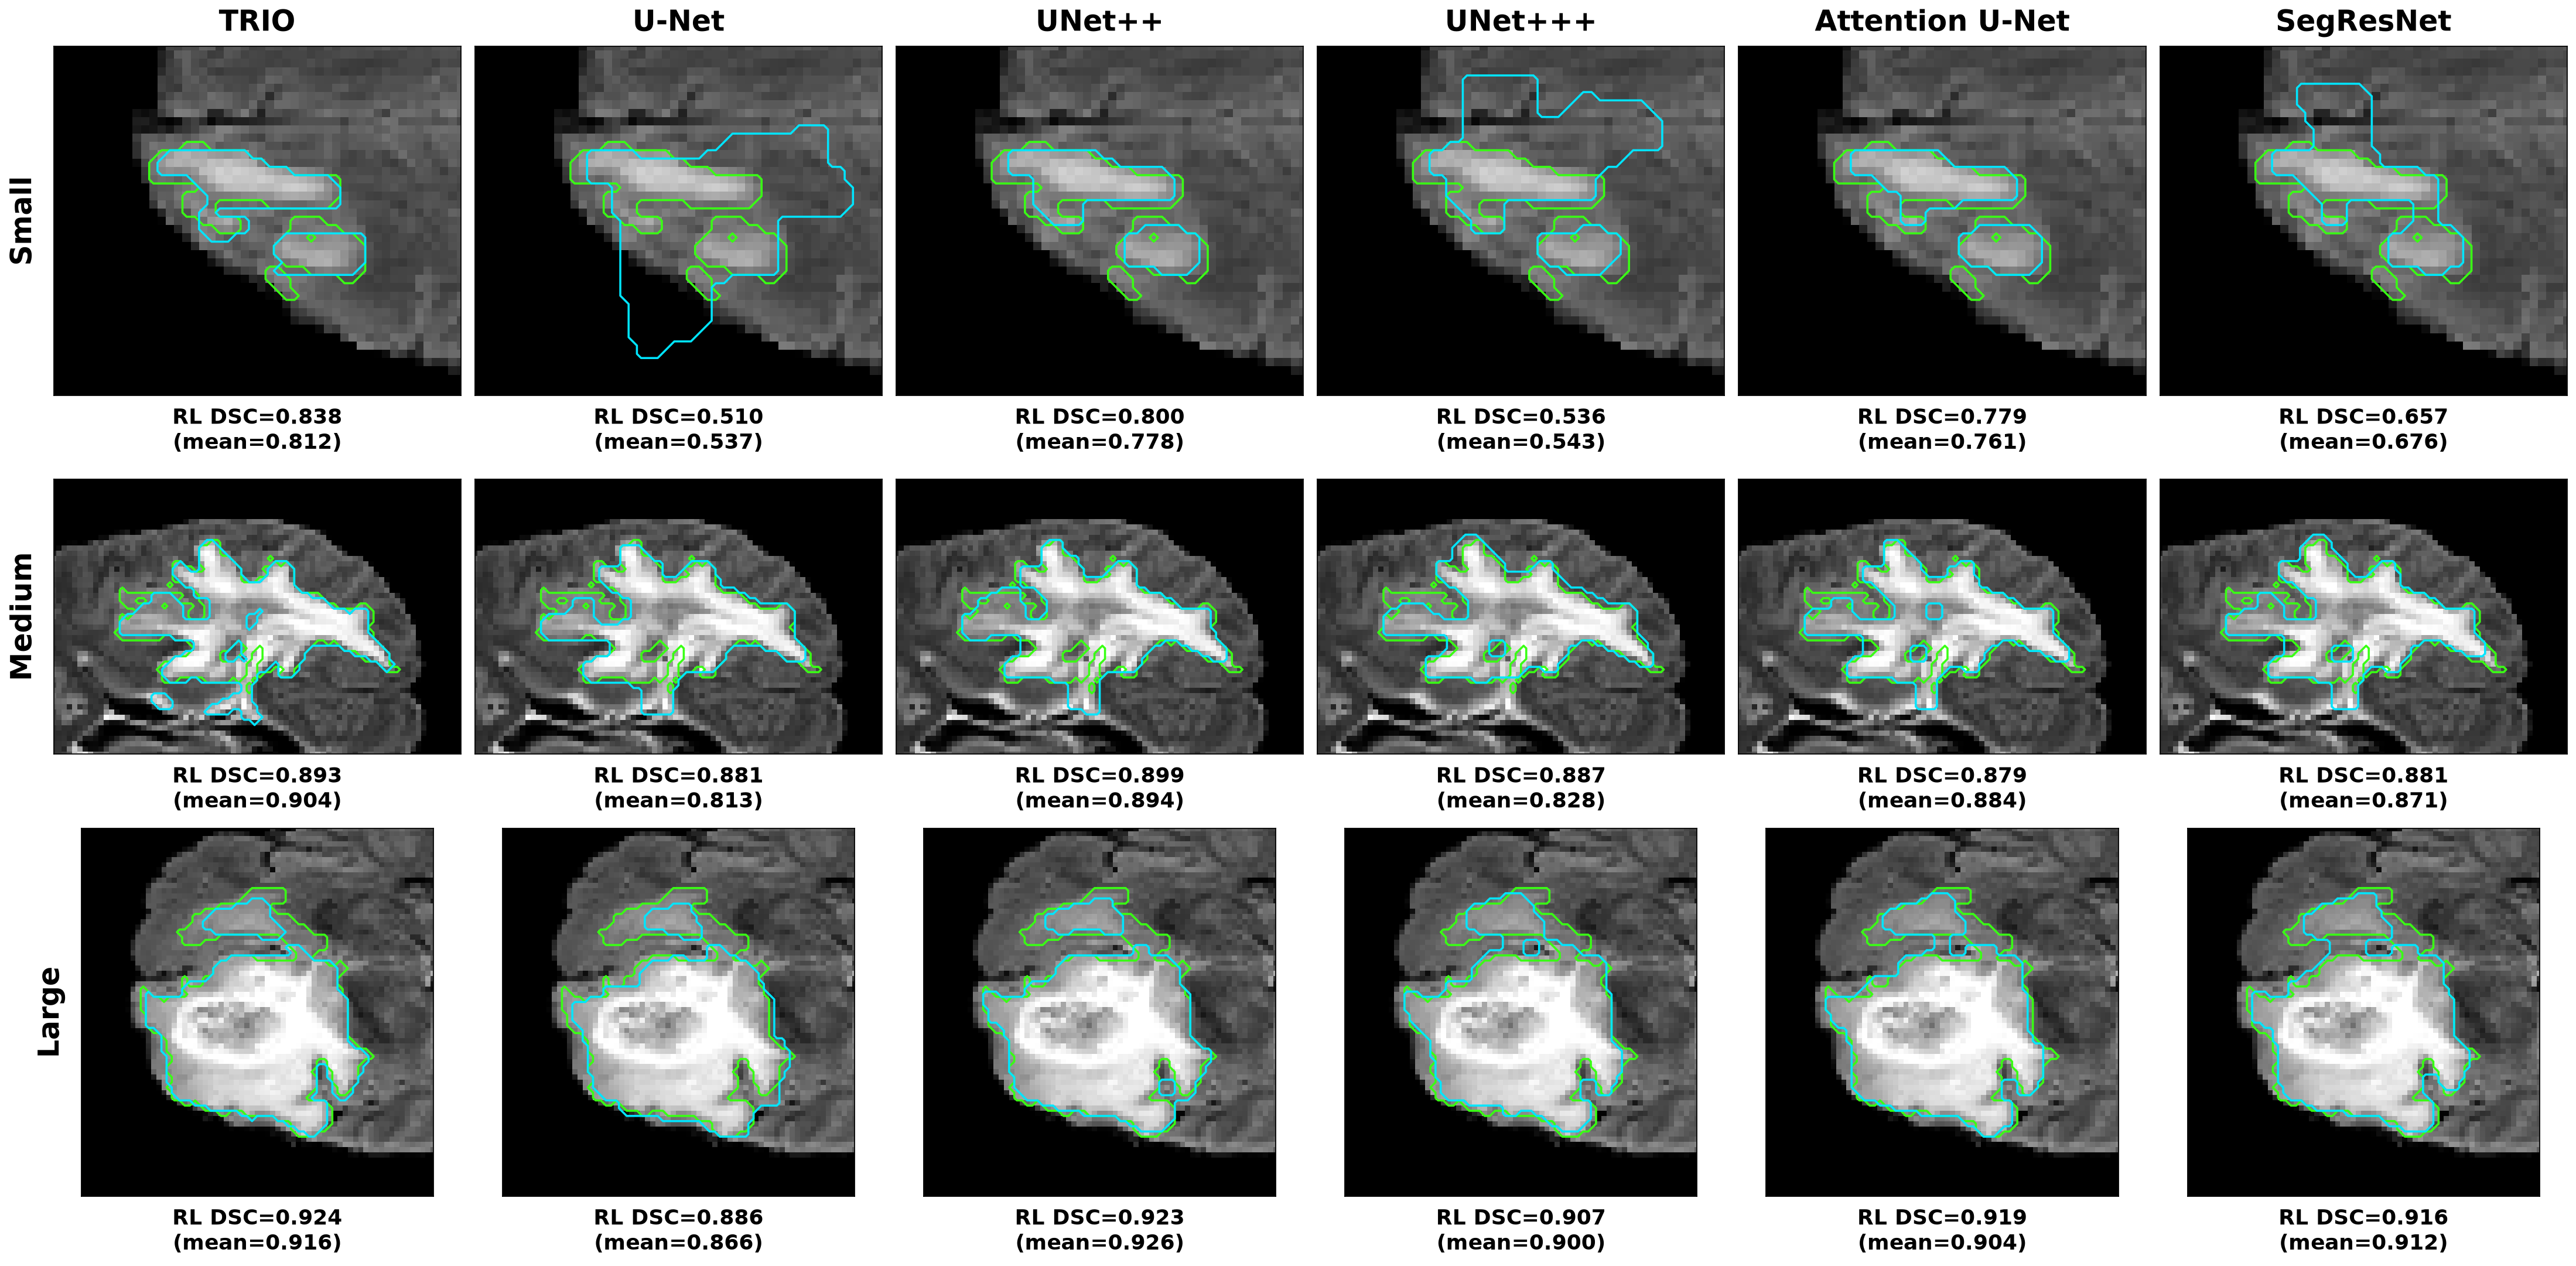
\includegraphics[width=\textwidth]{single_backbone_ppo_grid.png}
\caption{미사용 48명에서 고른 단면. 열은 TRIO와 단일 백본 PPO 다섯 개, 행은 정답 면적이다. 초록은 정답, 청록은 예측이다. 칸 아래 평균은 표~\ref{tab:single}의 슬라이스 평균이다.}
\label{fig:single}
\end{figure}

\subsection{주장 범위}
표~\ref{tab:locked}은 고정 임계값 Stage~2와의 짝비교이고, 표~\ref{tab:retune}는 검증 60명으로 임계값을 다시 고른 Stage~2와의 짝비교이다. 두 표 모두 같은 분류기와 전문가의 출력이다. 표~\ref{tab:baselines}와 표~\ref{tab:bysize}은 검증에서 임계값을 고른 2차원 각색과의 환자 평균 비교이며, 방법 간 짝 차이의 구간은 없다. 네 표 모두 3차원 BraTS 점수, 소형 종양만 있는 환자군의 성능, 짝이 맞는 HD95 개선을 뜻하지 않는다. 표~\ref{tab:single}은 같은 가중치의 851명 환자 평균이 아니라, 48명 표본 2{,}754장의 슬라이스 평균이다. 그 열의 PPO는 경계 띠가 아니라 섹터 이동이다. 학습에 쓴 280명의 Stage~2 예측은 그 환자를 이미 학습한 전문가의 출력이다. 접힘 밖 예측으로 정책을 다시 학습하지는 않았다. 851명의 전문가는 그 환자를 학습하지 않았으므로, 표~\ref{tab:locked} 자체는 같은 초기 마스크에서의 짝비교이다.

\section{고찰}

경계 띠로 수정 범위를 제한한 뒤 DSC의 환자 평균이 올랐다. 정책은 띠 밖의 전문가 레이블을 그대로 두고, 애매한 확률과 경계 근처만 고친다. 차이의 크기는 구간마다 다르다. 작은 단면의 초기 DSC가 0.7579로 가장 낮고 짝 차이도 $+0.0354$로 가장 크며, 재선택 Stage~2 대비로도 $+0.0251$로 가장 크다. 큰 단면은 초기 DSC가 높아 띠 보정의 여유가 작다.

외부 비교는 한 방향으로 정리되지 않는다. 작은 단면 DSC는 제안 방법이 높고, 전체 DSC는 NVAUTO 각색과 구간이 겹쳐 비슷하다. 중형·대형 DSC와 빈 마스크를 뺀 HD95 평균은 NVAUTO 각색이 더 좋다. 고정 Stage~2 대비 PPO는 재현율을 0.820에서 0.860으로, 정밀도를 0.883에서 0.892로 올렸다. 겹침 이득은 주로 띠에서 놓친 종양 픽셀을 켜는 결정에서 왔을 가능성이 크다. 이 해석은 픽셀 단위 오류 분해를 대체하지 않는다.

FLAIR 제약은 마지막 스텝에만 있고, 띠 평균보다 밝으면 종양이라는 선행을 넣는다. 밝은 부종 경계에는 맞을 수 있으나 어두운 괴사에는 맞지 않을 수 있다. 앞 스텝에서 바뀐 픽셀은 이 규칙으로 모두 되돌려지지 않는다. 분류기와 정답 크기가 다른 슬라이스 19.9\%에서는 학습 때와 다른 전문가의 오차를 수정한다. 분류기를 개선하면 이 비율은 줄 수 있으나, 본 실험에서 그 효과는 재지 않았다.

임계값만 다시 고르면 표~\ref{tab:locked} 이득의 약 28\%가 설명되지만, 재현율을 얻는 만큼 정밀도를 잃는다. PPO는 같은 확률 맵에서 둘을 함께 올렸고, 재선택 Stage~2보다도 $+0.0193$ 높다. 따라서 이득의 대부분은 임계값 위치가 아니라 띠 안의 픽셀별 결정에서 나온다.

단일 백본 다섯 개는 같은 280명으로 학습했지만, 크기별 전문가와 경계 띠를 쓰지 않는다. 48명 표본의 슬라이스 평균에서 소형 DSC는 TRIO 0.812에 비해 U-Net 0.537, UNet+++ 0.543까지 떨어진다. UNet++는 중형 0.894, 대형 0.926으로 이 표본의 TRIO와 같은 자리에 있다. 이 비교는 851명 환자 평균이 아니므로 표~\ref{tab:locked}의 0.8604와 한 줄에 두지 않는다.

비교에서 빠진 것도 분명히 둔다. 고정 임계값 0.80/0.80/0.50은 이전 210명 풀에서 정했고, 그 풀의 148명이 확정 평가에 들어 있다. 가중치와 띠 설계는 이번 개발 400명에서 정했지만, 이 임계값은 그 148명을 본 뒤 정해진 값이다. 표~\ref{tab:retune}의 재선택 임계값은 검증 60명에서만 골랐고, 그 비교에서도 PPO의 이득이 남는다. 다만 PPO는 고정 임계값 마스크로만 학습했고, 재선택 마스크로 다시 학습한 정책은 평가하지 않았다. 반전 증강은 제안 방법에만 있다. 베이스라인은 2차원 각색 한 시드이며 대회 제출의 앙상블이 아니다. HD95는 픽셀 단위이고, 원본 간격의 밀리미터 거리나 3차원 표면 거리로 환산하지 않았다. 정책 학습은 한 번의 실행이다.

\section{결론}

크기별 전문가와 하나의 경계 띠 PPO를 BraTS 2021의 미사용 851명에 적용하면, 분류기가 전문가를 고르고 임계값이 0.80/0.80/0.50인 Stage~2보다 2차원 슬라이스 DSC의 환자 평균이 0.8337에서 0.8604로 올랐다. 환자 짝 차이 $+0.0267$의 95\% CI는 0을 포함하지 않는다. 검증 60명으로 임계값을 다시 고른 Stage~2(0.8411)와 비교해도 $+0.0193$(95\% CI $0.0184$--$0.0202$)이 남는다. 학습과 에폭 선택은 정답 면적 라우팅이고, 이 평가는 분류기 라우팅이다. 같은 집계에서 KAIST 각색의 DSC는 0.8463, NVAUTO 각색은 0.8576으로, 제안 방법과 NVAUTO 각색은 비슷한 수준이다. 빈 마스크를 뺀 HD95 평균과 중형·대형 DSC는 NVAUTO 각색이 더 낮다.

이 결과는 고정된 초기 분할의 경계 띠를 고쳤을 때의 2차원 환자 평균이다. 수정 범위는 경계 $\pm2$픽셀과 확률 $[0.35,0.65]$인 픽셀이다. 같은 학습 환자로 백본 하나와 섹터 PPO만 둔 48명 표본에서는 소형 슬라이스 평균 DSC가 U-Net 0.537, UNet+++ 0.543까지 내려가고, 그 표본의 TRIO는 0.812이다. 이 표본 평균은 위 851명 환자 평균과 다른 집계다.

\begin{thebibliography}{10}
\bibitem{ronneberger2015}
Ronneberger, O., Fischer, P., Brox, T.: U-Net: Convolutional networks for biomedical image segmentation. In: MICCAI. pp. 234--241 (2015)

\bibitem{zhou2019}
Zhou, Z., Siddiquee, M.M.R., Tajbakhsh, N., Liang, J.: UNet++: Redesigning skip connections to exploit multiscale features in image segmentation. IEEE Trans. Med. Imaging \textbf{39}(6), 1856--1867 (2019)

\bibitem{myronenko2018}
Myronenko, A.: 3D MRI brain tumor segmentation using autoencoder regularization. In: BrainLes (MICCAI). pp. 311--320 (2018)

\bibitem{lou2023}
Lou, A., Guan, S., Loew, M.: CaraNet: Context axial reverse attention network for segmentation of small medical objects. J. Med. Imaging \textbf{10}(1), 014005 (2023)

\bibitem{schulman2017}
Schulman, J., Wolski, F., Dhariwal, P., Radford, A., Klimov, O.: Proximal policy optimization algorithms. arXiv:1707.06347 (2017)

\bibitem{baid2021}
Baid, U., et al.: The RSNA-ASNR-MICCAI BraTS 2021 benchmark on brain tumor segmentation and radiogenomic classification. arXiv:2107.02314 (2021)

\bibitem{luu2021}
Luu, H.M., Park, S.H.: Extending nn-UNet for brain tumor segmentation. arXiv:2112.04653 (2021)

\bibitem{myronenko2021}
Myronenko, A., Hatamizadeh, A., et al.: Redundancy reduction in semantic segmentation of 3D brain tumor MRIs. arXiv:2111.00742 (2021)

\bibitem{liao2020}
Liao, X., Li, W., Xu, Q., Wang, X., Jin, B., Zhang, X., Zheng, Y.: Iteratively-refined interactive 3D medical image segmentation with multi-agent reinforcement learning. In: CVPR. pp. 9394--9402 (2020)

\bibitem{furuta2020}
Furuta, R., Inoue, N., Yamasaki, T.: PixelRL: Fully convolutional reinforcement learning with action-successor representation for image processing. IEEE Trans. Multimedia (2020)
\end{thebibliography}

\end{document}
